%-----------------------------------------------------------------------------
%
%               Template for sigplanconf LaTeX Class
%
% Name:         sigplanconf-template.tex
%
% Purpose:      A template for sigplanconf.cls, which is a LaTeX 2e class
%               file for SIGPLAN conference proceedings.
%
% Guide:        Refer to "Author's Guide to the ACM SIGPLAN Class,"
%               sigplanconf-guide.pdf
%
% Author:       Paul C. Anagnostopoulos
%               Windfall Software
%               978 371-2316
%               paul@windfall.com
%
% Created:      15 February 2005
%
%-----------------------------------------------------------------------------


\documentclass[preprint]{sigplanconf}

% The following \documentclass options may be useful:
%
% 10pt          To set in 10-point type instead of 9-point.
% 11pt          To set in 11-point type instead of 9-point.
% authoryear    To obtain author/year citation style instead of numeric.

\usepackage{amsmath}
\usepackage{array}
\usepackage{graphicx}
\usepackage[utf8]{inputenc}

\usepackage[unicode=true]{hyperref}
\usepackage{color}

\newcommand{\TODO}[1]{\(\spadesuit\){\bf TODO:} {\bf \color{red} #1}\\}

\begin{document}

\conferenceinfo{Haskell Symposium '13}{2013-09-23, Boston} 
\copyrightyear{2013} 
\copyrightdata{[to be supplied]} 

\titlebanner{Submitted to Haskell Symposium 2013}        % These are ignored unless
%\preprintfooter{short description of paper}   % 'preprint' option specified.

\title{An EDSL approach to High Performance Haskell programming}
%\subtitle{Subtitle Text, if any}

%% %% \authorinfo{Johan Ankner}{}{}
   %% %% \authorinfo{Josef Svenningsson}{}{}
   %% 
\authorinfo{Johan Ankner}
           {}
           {skuggi@gmail.com}

\authorinfo{Josef Svenningsson}
           {Chalmers University of Technology}
           {josef.svenningsson@chalmers.se}

\maketitle

\begin{abstract}
This paper argues for a new methodology for writing high performance
Haskell programs by using Embedded Domain Specific Languages. 

We exemplify the methodology by describing a complete library,
meta-repa, which is a reimplementation of parts of the repa
library. The paper describes the implementation of meta-repa and
contrasts it with the standard approach to writing high performance
libraries. We conclude that even though the embedded language approach
has an initial cost of defining the language and some syntactic
overhead it gives a more natural programming model, stronger
performance guarantees, better control over optimizations, simpler
implementation of fusion and inlining and allows for moving type level
programming down to value level programming in some cases. We also
provide benchmarks showing that meta-repa is as fast, or faster, than
repa.

Furthermore, meta-repa also includes push arrays and we demonstrate
their usefulness for writing certain high performance kernels such as
FFT.
\end{abstract}

%\category{CR-number}{subcategory}{third-level}

%\terms
%term1, term2

\keywords
EDSL, array programming, optimization, meta programming

\section{Introduction}

In recent years the Haskell community has developed an increasing
interest in writing programs which perform well. Much thanks to the
advancements of optimizations and language design focused on efficiency
in GHC, the Haskell community now enjoys several high-performance
libraries and it is quite possible to write efficient code in Haskell.

In this paper we introduce a new methodology to take high performance
Haskell programming to a new level, by use an embedded domain specific
language approach. Embedded domain specific languages (EDSLs), and in
particular embedded compilers, have been very popular in Haskell for
quite some time now and has proven very effective for formulating good
abstractions which both provides a natural programming model and
efficient code generation. Up until now, high performance EDSLs has been
generating code for targets such as C, CUDA and VHDL. Our methodology
aims to bring these advantages to writing high performance Haskell
programs, by generating efficient Haskell code.

By formulating an EDSL and thereby restricting the language somewhat,
many optimization problems become much simpler. As we will demonstrate
in this paper, it is possible guarantee that all types are unboxed,
every function inlined and all array computations fused. These things
can be achieved by still allowing a rich and expressive programming
interface.

To demonstrate the viability of our methodology, this paper presents a
case study, meta-repa, which is a reimplementation of parts of the repa
library (Keller et al. 2010). The library meta-repa (the name comes from
the fact that it implements repa using meta-programming techniques) is
described in some detail to show how achieve the advantages of EDSLs
when used for Haskell programming. We include measurements against repa
to show that the code generated from meta-repa can indeed compete with a
well-designed and mature, high-performance library.

The contributions of the paper are as follows:

\begin{itemize}
\item
  We present a new methodology for writing high performance Haskell
  programs. We argue for using an embedded domain specific language and
  generate Haskell from that language. Programming in the domain
  specific language will be easier for the end user because the language
  can be given a semantics which matches the problem domain.

  Furthermore, several aspects of the implementation of the library
  becomes simpler when using the embedded language approach. In
  particular, many things that are done of the type level can now be
  done the value level.
\item
  We show how we use the technique of combining deep and shallow
  embeddings, building on the work in (Svenningsson and Axelsson 2012),
  to implement arrays. This technique helps limit the size of the core
  language, implement fusion for arrays for free and give strong
  optimization guarantees.
\item
  We demonstrate a complete case-study, meta-repa, showing the benefits
  of our approach. It is a reimplementation of the repa (Keller et al.
  2010) library using the embedded language approach. We explain the
  implementation in section \ref{sec:impl}. Section \ref{sec:benchmarks}
  presents benchmarks showing that meta-repa is on par with, and
  sometimes faster than repa.
\item
  Instead of one array type we have two. We have included Push arrays
  (Claessen, Sheeran, and Svensson 2012) in our implementation. The
  result is a simpler implementation of many array operations including
  stencil computations and although the user of our library must now use
  two different types of arrays we consider the resulting API to be
  easier to use. We explain the details in section \ref{sec:push}.
\end{itemize}

The reposity containing the code for meta-repa can be found at:
\url{http://github.com/jankner/meta-repa}

\section{Programming in meta-repa}

\label{sec:programming}

The basic unit of a meta-repa program are values of the type
\texttt{Expr a}, which represent expressions in the core language. For
example, a simple numeric expression can be written using the standard
Num instance:

\begin{verbatim}
e :: Expr Int
e = 10*5+2
\end{verbatim}

Functions are written as normal Haskell functions over \texttt{Expr}s.
For example, a simple numeric function:

\begin{verbatim}
f :: Expr Int -> Expr Int -> Expr Int
f a b = a*a - b
\end{verbatim}

Some examples of core language constructs:

\begin{verbatim}
if_ :: Computable a => Expr Bool -> a -> a -> a

iterateWhile :: Computable a 
             => (a -> Expr Bool)
             -> (a -> a) 
             -> a
             -> a
\end{verbatim}

Note that polymorphic arguments use the class \texttt{Computable} rather
than being of type \texttt{Expr a}. The \texttt{Computable} class allows
the programmer to write code as if certain Haskell constructs are part
of the core language. For example, it is more convenient to work with
the type \texttt{(Expr Int, Expr Double)} rather than
\texttt{Expr (Int, Double)} because the former can be constructed and
deconstructed with Haskell's ordinary tuple syntax. \texttt{Computable}
handles the tupling and untupling in the core language automatically.

The library for array computations are implemented as a shallow
embedding on top of the core language. There are two different types of
arrays in meta-repa, Pull arrays and Push arrays. Pull arrays correspond
to the delayed array representation in repa. Push arrays are a different
kind of delayed representation that supports a different set of
operations. Pull arrays are discussed further in \ref{sec:shallow}. Push
arrays are discussed in detail in \ref{sec:push}. The \texttt{Shape}
type is used to represent array indices of varying dimensionality. The
type parameter determines the dimension of the index. For example the
type paremeter \texttt{DIM2} indicates a two-dimensional index. This
works much the same as in repa, though it is implemented in a slightly
different way. This is discussed in more detail in section
\ref{sec:shape}.

The library includes functions for manipulating arrays. Many of them
correspond to list functions found in the Prelude. Both array types also
have a Functor instance.

Here are some examples of functions for Pull arrays that exist in the
library:

\begin{verbatim}
zipWith :: (a -> b -> c) 
        -> Pull sh a -> Pull sh b -> Pull sh c

fromFunction :: (Shape sh -> a) 
             -> Shape sh 
             -> Pull sh a

foldS :: (Computable a, Computable b)
      => b
      -> (a -> b -> b)
      -> Pull (sh :. Expr Length) a
      -> Pull sh b
\end{verbatim}

\texttt{fromFunction} takes an index function and an extent and
constructs a Pull array. \texttt{foldS} performs a sequential fold on
the outer dimension of an array with at least one dimension, and returns
an array that has one less dimension than the input.

In figure \ref{fig:comparison} is a comparison between the
implementation of a function in repa and meta-repa. The fucntion
\texttt{step} is a part in calculating the Mandelbrot set. It calculates
$z_{i+1} = z_i + c$ for a given complex plane, where $c$ comes from the
first argument and $z_i$ comes from the second argument.

\begin{figure*}
\begin{tabular}{p{\columnwidth} | p{\columnwidth}}

\begin{verbatim}
type Complex = (Double, Double)
type ComplexPlane r = Array r DIM2 Complex
type StepPlane r = Array r DIM2 (Complex,Int)

step :: ComplexPlane U 
     -> StepPlane U
     -> IO (StepPlane U)
step cs zs = computeP $ zipWith stepPoint cs zs
  where
    stepPoint :: Complex
              -> (Complex,Int)
              -> (Complex,Int)
    {-# INLINE stepPoint #-}
    stepPoint !c (!z,!i) =
        if magnitude z' > 4.0 
          then (z,i)
          else (z',i+1)
      where
        z' = next c z
    next :: Complex -> Complex -> Complex
    {-# INLINE next #-}
    next !c !z = c + (z * z)
\end{verbatim}
&
\begin{verbatim}
type Complex = (Expr Double, Expr Double)
type ComplexPlane = Pull DIM2 Complex
type StepPlane = Pull DIM2 (Complex, Expr Int)

step :: ComplexPlane 
     -> StepPlane
     -> StepPlane
step cs zs = forcePull $ zipWith stepPoint cs zs
  where
    stepPoint :: Complex 
              -> (Complex,Expr Int)
              -> (Complex,Expr Int)
    stepPoint c (z,i) =
        if_ (magnitude z' > 4.0)
          (z,i)
          (z',i+1)
      where
        z' = next c z
    next :: Complex -> Complex -> Complex
    next c z = c + (z * z)
\end{verbatim}
\end{tabular}
\caption{A comparison between programming in repa and meta-repa}
\label{fig:comparison}
\end{figure*}

The two code fragments are quite similar, with some details being
different . Here are the differences:

\begin{itemize}
\itemsep1pt\parskip0pt\parsep0pt
\item
  \texttt{Int} and \texttt{Double} becomes \texttt{Expr Int} and
  \texttt{Expr Double}.
\item
  meta-repa does not have an explicitily manifest array type. Instead,
  the forcePull function is used to write a Pull array to an underlying
  array and return a Pull array which reads from it.
\item
  The meta-repa code uses the function \texttt{if\_} rather than
  Haskell's \texttt{if then else}.
\item
  The repa code uses bang-patterns and INLINE pragmas to make sure that
  the worker functions are properly inlined and static. In meta-repa
  everything is inlined by default and it is completely static.
\end{itemize}

When you have written your meta-repa code it can be translated and
spliced into a module using Template Haskell. For example you might have
this meta-repa function in one module:

\begin{verbatim}

f :: Expr Int -> Expr Int -> Expr Int
f a b = sumS (enumFromTo a b)
\end{verbatim}

In another module which imports that function, the function can be
spliced in like this:

\begin{verbatim}

func :: Int -> Int -> Int
func = $(translate f)
\end{verbatim}

\subsection{Contract towards the programmer}

The library meta-repa comes with a set of guarantees towards the
programmer. These contracts helps the programmer understand the
efficiency of a particular program. They also show precisely when a
programmer can introduce abstraction without losing any performance.

\begin{itemize}
\item
  \emph{All types are monomorphised and unboxed}.

  In particular, expressions of type \texttt{Expr Int} will be compiled
  to \texttt{Int\#}, \texttt{Expr Float} to \texttt{Float\#}, pairs to
  unboxed pairs and so forth.

  The programmer is free to write polymorphic and overloaded code. But
  once the final Haskell code is generated, all types will be
  monomorphic and unboxed.
\item
  \emph{Every function is inlined by default}.

  In high performance code, inlining functions is the right default
  behaviour and generally increases the performance a lot. When the
  programmer wants to prevent inlining, for whatever reason, it is
  simple to create a locally defined function with the \texttt{let\_}
  combinator provided by our library.
\item
  \emph{Operations on arrays are fused automatically}.

  Our library has two types of arrays, \texttt{Pull} and \texttt{Push},
  and all operations working on only one of these types will always be
  fused, as will conversions from \texttt{Pull} to \texttt{Push}.
  However, conversions from \texttt{Push} to \texttt{Pull} are not
  fused. This exception might seem surprising but we explain why this is
  the right default in section \ref{sec:push} on Push arrays.

  Fusion can easily be prevented by inserting the function
  \texttt{force}, which will store the array to memory. This follows the
  design used in Feldspar and repa.
\item
  \emph{Common subexpression elimination and code motion are applied
  extensively on the program}.

  GHC already does these optimizations to some extent but because of the
  domain specific nature of our library, we can apply these
  optimizations more extensively than GHC.
\end{itemize}

These guarantees and optimizations are possible and practical because we
are working with a limited domain specific language. When compiling a
general purpose language, many program optimizations often turn out to
be pessimizations for certain classes of programs. By constructing a
smaller language we've made the problem of optimizing programs much
easier.

In the next sections we will describe how our implementation achieves
these guarantees. Many of them come for free, as a side effect of how
we're representing programs.

\section{Implementation of meta-repa}

\label{sec:impl}

\begin{figure*}[t]
\center
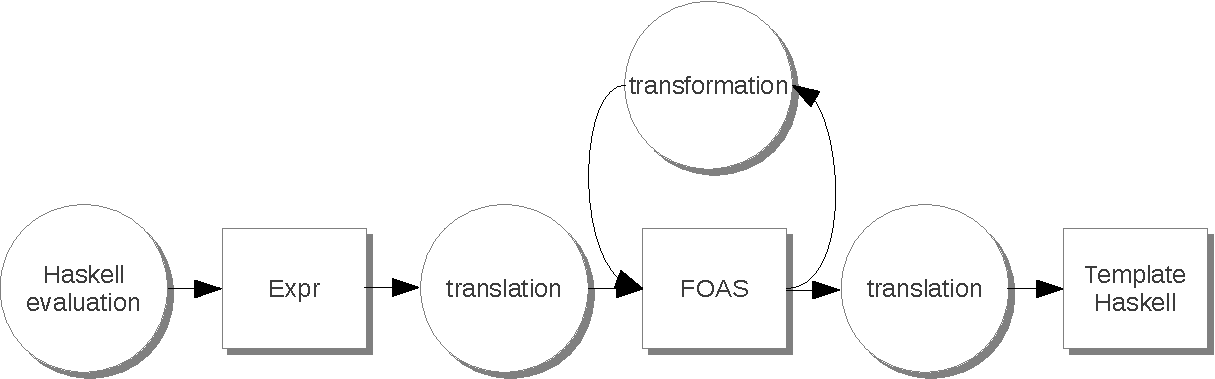
\includegraphics[scale=0.8]{meta.pdf}
\caption{The compilation pipeline for meta-repa programs}
\label{fig:pipeline}
\end{figure*}

This section explains most of the implementation of meta-repa. Some
details, in particular the use of Push arrays are explained in section
\ref{sec:push}.

Programs in meta-repa are in fact program generators. When meta-repa
functions are run they produce abstract syntax trees which are then
further translated and transformed. Figure \ref{fig:pipeline} gives an
overview of this process. Boxes represents abstract syntax trees and
circles represents transformations and translations. First the code
within the Template Haskell splice is run. This will compute a term of
type \texttt{Expr}, a GADT which ensures type safety of program by
construction. Since all functions defined using the meta-repa library
are really Haskell functions they will simply compute new syntax trees.
The net effect will be that the code in the functions will be inlined
(unless prevented by the programmer). The inlining happens purely as a
result of Haskell's evalutation, there is no code in the meta-repa
library which performs any inlining.

The type \texttt{Expr} uses higher order abstract syntax to represent
programs. This representation is convenient for programming with but
somewhat less ideal for rewriting programs. The AST is therefore
converted into a first order representation, which we will refer to as
\texttt{FOAS}. A possible implementation would have been to skip the
\texttt{Expr} type and generate the first order representation directly.
We have kept the higher order represtentation partly because it helps
maintain the type safety of the implementation and partly because it
allows us to write a well typed, tagless interpreter.

Two optimizations are performed on the \texttt{FOAS} representation:
common subexpression elimination (CSE) and code motion. CSE finds
identical subexpressions and shares their computation so that it only
happens once. The transformation is selective with exactly what
subexpressions to share. We found in measurements that the generated
code was faster if most small subexpressions were left unshared. The
code motion transformation moves code up the syntax tree to that it is
computed as early as possible. It also moves constant expressions out of
loops.

Another popular way to achieve CSE is to represent the syntax tree as a
DAG and thereby get sharing as a side effect of the representation.
We've chosen to use a simpler tree based representation with an explicit
\texttt{let} construct for sharing which allows us to make local
decisions about what to share and what to duplicate.

All the translations and transformations explained above are performed
by the \texttt{transform} function mentioned in section
\ref{sec:programming}. After the \texttt{FOAS} representation is added
the \texttt{transform} function adds a wrapper around its argument
giving it a type which makes it easier to call from Haskell. Then, as a
last step the code is translated to Template Haskell and spliced into
the module by GHC.

We would like to point out that the use of Template Haskell is just a
matter of convenience and not of fundamental importance. Another
possibility would have been to write the generated Haskell code to a
separate file which the programmer would then have to compile
separately.

\subsection{Core Language(s)}

\begin{figure}
\begin{verbatim}
data Expr a where
  Var   :: Int -> Expr a
  Value :: a -> Expr a

  Lambda :: Type a -> (Expr a -> Expr b)
         -> Expr (a -> b)
  App :: Expr (a -> b) -> Expr a -> Expr b

  Binop :: Binop a -> Expr a -> Expr a -> Expr a
  Equal :: Eq a => Expr a -> Expr a -> Expr Bool
  NotEqual :: Eq a => Expr a -> Expr a -> Expr Bool

  Tup2 :: Expr a -> Expr b -> Expr (a,b)
  Fst :: Expr (a,b) -> Expr a
  Snd :: Expr (a,b) -> Expr b

  Let :: Expr a -> (Expr a -> Expr b) -> Expr b
  If :: Expr Bool -> Expr a -> Expr a -> Expr a
  IterateWhile :: Expr (s -> Bool) -> Expr (s -> s)
               -> Expr s -> Expr s

  ReadIArray :: Storable a =>
                Expr (UArray Int a) -> Expr Int
             -> Expr a
  ArrayLength :: Storable a =>
                 Expr (UArray Int a) -> Expr Int

  Return :: Expr a -> Expr (IO a)
  Bind   :: Expr (IO a) -> Expr (a -> IO b)
         -> Expr (IO b)

  WhileM :: Expr (s -> Bool) -> Expr (s -> s)
         -> Expr (s -> IO ()) -> Expr s
         -> Expr (IO ())

  RunMutableArray :: Storable a =>
                     Expr (IO (IOUArray Int a))
                  -> Expr (UArray Int a)

  NewArray   :: Storable a =>
                Type a -> Expr Int
             -> Expr (IO (IOUArray Int a))
  ReadArray  :: Storable a =>
                Expr (IOUArray Int a) -> Expr Int
             -> Expr (IO a)
  WriteArray :: Storable a =>
                Expr (IOUArray Int a)
             -> Expr Int -> Expr a -> Expr (IO ())
  ParM       :: Expr Int -> Expr (Int -> IO ())
             -> Expr (IO ())
\end{verbatim}
\caption{A representative subset of the \texttt{Expr} data type}
\label{fig:expr}
\end{figure}

The core language of meta-repa, represented by the \texttt{Expr} data
type, is a standard typed higher order abstract syntax representation
implemented using GADTs. A fragment with the most relevant constructs is
shown in Figure \ref{fig:expr}.

The first two constructors \texttt{Var} and \texttt{Value} are used for
compilation and evaluation and will never be present in trees produced
by code written in meta-repa.

The constructors \texttt{Lambda} and \texttt{App} together with the
constructs for binary operators, comparisons and tuples form a small
functional language for arithmetic and tests which is useful for
efficient scalar computations.

The \texttt{Let} construct is used for explicit sharing in the syntax
tree. It is exposed to the programmer via the \texttt{let\_} function
which can be used to prevent inlining and explicitly share computations.
It is worth pointing out that meta-repa does not employ observable
sharing (Claessen and Sands 1999) so no new \texttt{Let} constructors
are introduced when the program is represented by the \texttt{Expr}
type.

The constructor \texttt{If} and \texttt{IterateWhile} are unsurprising
control flow constructs for pure computations.

There are two types of in-memory arrays in the code language. These
arrays are not exposed to the programmer, they are instead used as
building blocks for the array types implemented as shallow embedding
which we explain in the next subsection. The two type of array in the
core language are always allocated in memory. One of the types is
\texttt{UArray} which represents pure arrays and the constructs
\texttt{ReadIArray} and \texttt{ArrayLength} can be used to query them.
There is no pure construct for creating pure arrays, instead they must
be created through destructive, monadic constructs which we turn to
next.

To begin with, the monadic construct contains the generic
\texttt{Return}, \texttt{Bind} and a looping construct, \texttt{WhileM}.
Then there are a few constructs for creating, reading and updating
mutable arrays. The \texttt{RunMutableArray} construct takes a monadic
computation and returns a pure array. In that way it is similar to the
ST monad (Launchbury and Peyton Jones 1994). Compared to the ST monad,
the state parameter in the type has been omitted, since there is no
construct corresponding to \texttt{runST} with a polymorphic return type
which could voilate safety by passing mutable arrays outside of the
scope of their monadic computation.

Finally, there is the parallel for-loop, \texttt{ParM}, which is the
construct for parallel computations. Currently it is possible to have a
\texttt{ParM} inside another\texttt{ParM} in the core language. However,
as we discuss in section \ref{sec:runtime}, our runtime system does not
allow this kind of nesting. We have not made any attempts at disallowing
nesting in the type system. Instead, the API to meta-repa is designed
such that nested parallel loops should never occur. This has affected
the Push array library (covered in section \ref{sec:push}); certain
combinators use a sequential loop where they could have used a parallel
loop in order to keep the parallelism flat.

There are a couple of things to note about the core language:

\begin{itemize}
\item
  It is monomorphic. Having a monomorphic language is important to be
  able to always generate unboxed Haskell code.

  A monomorphic core language does not stop the programmer from writing
  polymorpic programs or using overloading. Functions can be written
  which work for several different base types. The only restriction is
  that when compiling a meta-repa program, all types must be
  instantiated to monomorphic types.
\item
  It has a strict semantics. In order to get maximum performance and,
  again, to be able to unbox as much as possible we have chosen a strict
  semantics for meta-repa. It also fits better with the domain compared
  to lazy evaluation. When writing high performance Haskell one often
  has to resort to inserting calls to \texttt{seq} and using bang
  patterns to get strict code. None of that is necessary when
  programming in meta-repa due to its semantics.
\end{itemize}

The core language comes with an evaluation function which defines the
semantics. The evaluation function is straighforward to write. It is
also very useful for trying out the language during its development and
as a reference semantics to test the Template Haskell against.

As mentioned above, \texttt{Expr} is translated into a first order
representation, \texttt{FOAS}, which is used for transforming the
program. The type \texttt{FOAS} has all the same constructs as
\texttt{Expr} but in a first order representation with explicit
variables and explicit types which have been reified from the Haskell
types parameter for \texttt{Expr}. Below is the constructor for the pure
iteration construct in \texttt{FOAS}.

\begin{verbatim}
IterateWhile Type FOAS FOAS FOAS
\end{verbatim}

The first argument to \texttt{IterateWhile} is a value representing the
type of the state passed around during iteration.

\subsection{Shallow Embeddings for Arrays}

\label{sec:shallow}

The implementation of meta-repa follows the methodology of combining
deep and shallow embeddings descibed in (Svenningsson and Axelsson
2012). The type \texttt{Expr} is a deeply embedded core language which
contains all the language constructs necessary to generate efficient
code from any meta-repa program. On top of the core language there are
several shallow embeddings; in the case of meta-repa there are two types
of arrays which are implemented as shallow embeddings. Implementing
language constructs as shallow embeddings help keep the core language
small and allows for easy and lightweight experimentation with different
language constructs without having to add new constructors in the core
language and translation functions for those.

In meta-repa there are two constructs which are implemented as shallow
embeddings; arrays and monads. The monad provided by meta-repa is simply
called \texttt{M} and provides wrappers for all the monadic operations
in the core language. Implementing \texttt{M} as a shallow embedding has
the advantage of proving an instance of the \texttt{Monad} type class.
This instance enables the programmer to use do-notation and reuse all
the monadic combinators in the standard library. For the details of how
the shallow embedding for monads work we refer the reader to the paper
(Persson, Axelsson, and Svenningsson 2012).

Arrays are also implemented as shallow embeddings. While this is not a
new technique, we will present enough details about the implementation
in meta-repa to show how it contributes to writing high performance
Haskell programs. There are two kinds of arrays in meta-repa, but we
will focus on one of them here, Pull arrays, and leave the description
of the other kind, Push array, for section \ref{sec:push}. Pull arrays
are defined as follows:

\begin{verbatim}
data Pull sh a = Pull (Shape sh -> a) (Shape sh)
\end{verbatim}

Representing arrays as functions from index to value has become a
popular way due to its simple implementation and nice properties. In
particular, since every element is computed independently, it is very
easy to parallelize writing such arrays to memory.

Below are some examples for functions on Pull arrays:

\begin{verbatim}
instance P.Functor (Pull sh) where
  fmap f (Pull ixf sh) = Pull (f . ixf) sh

storePull :: (Computable a, Storable (Internal a)) =>
             Pull sh a
          -> M (Expr (MArray (Internal a)))
storePull (Pull ixf sh) = 
  do arr <- newArrayE (size sh)
     forShape sh (\i ->
       writeArrayE arr i
         (internalize (ixf (fromIndex sh i))))
     return arr

fromFunction :: (Shape sh -> a) -> Shape sh
             -> Pull sh a
fromFunction ixf sh = Pull ixf sh

index :: Pull sh a -> Shape sh -> a
index (Pull ixf s) = ixf

zipWith :: (a -> b -> c)
        -> Pull sh a -> Pull sh b -> Pull sh c
zipWith f (Pull ixf1 sh1) (Pull ixf2 sh2)
  = Pull (\ix -> f (ixf1 ix) (ixf2 ix))
         (intersectDim sh1 sh2)

traverse :: Pull sh a -> (Shape sh -> Shape sh')
         -> ((Shape sh -> a) -> Shape sh' -> b)
         -> Pull sh' b
traverse (Pull ixf sh) shFn elemFn
  = Pull (elemFn ixf) (shFn sh)

forcePull :: Storable a =>
             Pull sh (Expr a) -> Pull sh (Expr a)
forcePull p@(Pull ixf sh)
    = Pull (\ix -> ixf' arr ix) sh
  where
    ixf' arr ix = readIArray arr (toIndex sh ix)
    arr = runMutableArray (storePull p)
\end{verbatim}

A perhaps surprising thing about Pull arrays is that they can be made an
instance of the type class \texttt{Functor}. Polymorphic functions in
embedded languages typically need some form of class constraint.
However, the definition of Pull arrays is carefully chosen such that
they can work with any Haskell type. It is only when actually storing
the array, as in the \texttt{storePull} function, where there has to be
a constraint on the type of element in the Pull array. The function
\texttt{storePull} uses the constructs for mutable arrays to write the
Pull array to memory. The function \texttt{forShape} is a parallel
for-loop, defined in terms of \texttt{parM}, which goes through all
elements in the shape of the array in parallel.

The function \texttt{fromFunction} provides an easy way to create
arrays, it's simply an alias for the \texttt{Pull} constructor. The
\texttt{index} function provides a means for indexing into the array. A
slightly more involved example is \texttt{zipWith} which works much like
the standard function on lists with the same name. The slightly
non-trivial part is that the shape of the final array is the
intersection of the shapes of the input arrays.

The function \texttt{traverse} is directly ported from the repa library
and enables powerful transformations of arrays. The implementation of
meta-repa also contains many other functions for manipulating arrays
ported from the repa library.

A nice benefit of the way Pull arrays are represented and using the
embedded language approach is that fusion comes for free and is
guaranteed. Compiling meta-repa programs means producing a syntax tree
of type \texttt{Expr}. Since this type doesn't contain the type
\texttt{Pull} we have a static guarantee that all Pull arrays will be
statically eliminated. A very powerful guarantee indeed. The fact that
it happens purely as a side-effect of Haskell's evalutation is an added
bonus.

Although fusion is often what the programmer wants, there are occasions
when it is good to be able to disable it. An example is when an array
transformation uses the elements of the input array more than once. Then
the computation which produced the elements of the input array will be
duplicated, akin to call-by-name evaluation. In such situations it is
often better to write the array to memory. The function
\texttt{forcePull} can be used to achieve this.

\subsection{From type level to value level programming}

\label{sec:shape}

In repa, the type of shapes of an array is represented by a type class
and two singleton types as follows:

\begin{verbatim}
class Shape sh where
  ...

data Z = Z
data sh :. e = sh :. e

instance Shape Z where
  ...

instance Shape sh => Shape (sh :. Int) where
  ...
\end{verbatim}

In meta-repa, thanks to the meta programming approach, shapes can be
represented by an ordinary data type definiton.

\begin{verbatim}
data Z
data sh :. e

data Shape sh where
  Z :: Shape Z
  (:.) :: Shape sh -> Expr Length
       -> Shape (sh :. Expr Length)
\end{verbatim}

Defining the \texttt{Shape} type like a GADT makes programming with is a
lot more natural. Many of the functions which had to be implemented in
the \texttt{Shape} type class in repa can now be implemeted as ordinary
functions.

\begin{verbatim}
dim :: Shape sh -> Int
dim Z = 0
dim (sh :. _) = dim sh + 1

size :: Shape sh -> Expr Length
size Z         = 1
size (sh :. l) = size sh * l

toIndex :: Shape sh -> Shape sh -> Expr Index
toIndex Z _ = 0
toIndex (sh1 :. sh2) (i1 :. i2)
  = toIndex sh1 i1 * sh2 + i2

intersectDim :: Shape sh -> Shape sh -> Shape sh
intersectDim Z Z = Z
intersectDim (sh1 :. n1) (sh2 :. n2)
  = (intersectDim sh1 sh2 :. (min n1 n2))

inRange :: Shape sh -> Shape sh -> Shape sh
        -> Expr Bool
inRange Z Z Z = true
inRange (shL :. l) (shU :. u) (sh :. i)
  = l <= i && i < u && inRange shL shU sh
\end{verbatim}

Being able to program on the value level rather than the type level is
clear improvement for the implementation of the library. It makes the
code more readable and maintainable. Another small win is that the API
of meta-repa contains less class constraints, making the types easier to
read and comprehend.

\subsection{Runtime system}

\label{sec:runtime}

The library meta-repa relies on a small runtime system in order to set
up the parallel computations and distribute them over the available
processes. We have chosen to reuse the runtime system from repa by
simply calling the the appropriate low-level functions provided the
library. This has had a number of positive effects. First, the repa
library has a well-developed and mature runtime system which has been
used and improved over several years. Secondly, when doing measurements
to compare against repa, the runtime system is equal and eliminates a
lot of possible sources of differences which could affect the
benchmarks. Being able to share runtime system means that the
comparisons can focus on the generated code and the amount of
parallelism made available in the different libraries.

A downside to using the runtime system of repa is that it only handles
flat parallelism. This means that it is not possible to nest the
\texttt{ParM} construct in the core language and some care has gone into
designing the API in meta-repa to avoid nesting. However, nested
parallelism is a much harder problem than flat parallelism and
developing a completely new runtime for meta-repa would have been
outside the scope of the project.

\section{Push arrays}

\label{sec:push}

The programmers interface in meta-repa is heavily inspired by repa, but
some things have been consiously made different. The most significant
divergence is the choice of having two kinds of arrays.

In meta-repa there are two types of arrays, delayed arrays. One of these
types, Pull arrays, were already presented in section \ref{sec:shallow}.
The other type is Push arrays, a notion originally introduced in
(Claessen, Sheeran, and Svensson 2012). Push arrays shares many
significant properties with Pull arrays: they can be fused just as
easily, are efficiently parallelizeable, and have a \texttt{Functor}
instance.

However, Push arrays are also in many ways complementary to Pull arrays.
The two types have different strengths:

\begin{itemize}
\item
  Pull arrays can be indexed efficiently and by extension can also be
  decomposed into subarrays. Pull arrays also supports pointwise
  zipping.
\item
  Push arrays can efficiently be concatenated. Futhermore, they allow
  sharing computations between different array elements and generating
  code which writes multiple array elements per loop interation.
\end{itemize}

It's worth noting that both Pull- and Push arrays can be altered to
efficiently support some of the features that they lack, when defined in
their simplest form. However, based on our experience, these alterations
lose the strong optimization guarantees; either fusion is lost, or
sometimes the generated code is slow. In meta-repa we have specifically
chosen to keep the implementation of the arrays simple and to provide
strong guarantees towards the programmer about what optimizations can be
expected.

Giving a full account of Push arrays falls outside the scope of this
paper. The interested reader is refered to (Claessen, Sheeran, and
Svensson 2012) where Push arrays were introduced. However, we will
present enough detail to get an appreciation for why they are useful for
the purpose of high performance Haskell programming.

Push arrays are implemented as follows:

\begin{verbatim}
data Push sh a = 
  Push ((Shape sh -> a -> M ()) -> M ()) (Shape sh)
\end{verbatim}

The second argument to the \texttt{Push} constructor is the extent of
the array. The first argument is a monadic computation (using the
\texttt{M} monad introduced in section \ref{sec:shallow}) which, when
run, will write the array to memory. We refer to this computation as the
kernel of the array. The kernel is parameterized by the operation used
to write to memory. Parameterizing over the writing operation is what
gives Push arrays their flexibility.

Here are some example functions on Push arrays.

\begin{verbatim}
enumFromTo :: Expr Int -> Expr Int
           -> Push (Z :. Expr Int) (Expr Int)
enumFromTo f t = Push loop (Z :. t - f + 1)
  where loop w = parM (t - f + 1) (\i ->
                   w (Z :. i) (i + f)
                 )

instance Functor (Push sh) where
  fmap f (Push m sh) = Push n sh
    where n w = m (\i a -> w i (f a))

(+.+) :: Push (sh:.Expr Length) a
      -> Push (sh:.Expr Length) a
      -> Push (sh:.Expr Length) a
(Push m1 (sh1:.l1)) +.+ (Push m2 (sh2:.l2))
    = Push m (sh1:.(l1 + l2))
  where m k = m1 k >>
              m2 (\(sh:.i) a -> k (sh:.(i+l1)) a)

force :: Storable a =>
         Push sh (Expr a)
      -> Push sh (Expr a)
force (Push f l) = Push f' l
  where f' k =
    do arr <- newArrayE (size l)
       f (\sh a ->
            writeArrayE arr (toIndex l sh) a)
       forShape l $ \i -> do
         a <- readArrayE arr i
         k (fromIndex l i) a
\end{verbatim}

The function \texttt{enumFromTo} is similar to the standard Haskell
function on lists with the same name. The kernel \texttt{loop} is
defined in terms of a parallel for-loop which writes each element.

Just like Pull arrays, Push arrays can be made an instance of the type
class \texttt{Functor} as shown in the code above. The kernel of the
result array simply calls the kernel of the argument array but modifies
the write function such that the elements get transformed before being
written.

The operator \texttt{+.+} is a good example of the benefits with Push
arrays. It defines concatenation along the final dimension of two Push
arrays. (The arrays must have the same size in all the other dimensions,
something which is not checked.) The kernel of the resulting Push array
is simply sequential composition of the kernels for the two argument
arrays. In the common case this will mean that the final array is
written using two loops, each writing to its own part of the array. This
should be compared the code generated from concatenation on Pull array,
which is a single loop containing a branch which checks which argument
array to read from. Concatenation for Push arrays has effectively moved
the conditional out of the loop, a big win in term of performance. It
should be added that an even better implementation of concatenation
would have used parallel composition instead of sequential composition.
However, our current runtime system doesn't support that. There is still
room for improvements.

Finally, the function \texttt{force} shows how Push arrays are written
to memory. It can be used by the programmer to prevent fusion and make
sure that an array is written to memory. The kernel of the resulting
array allocates a new in-memory array and calls the kernel of the input
array with a write function as a parameter which writes all the elements
to the newly allocated array. It then iterates through the array in
memory writing all the elements using the write function parameter.

Interoperating Pull arrays and Push arrays is an interesting story. Pull
arrays can easily be converted into Push arrays in a way that preserves
fusion. In meta-repa the function \texttt{toPush} is used for this
purpose:

\begin{verbatim}
toPush (Pull ixf sh) = Push m sh
  where m k = forShape sh (\i ->
                let ish = fromIndex sh i
                in  k ish (ixf ish)
              )
\end{verbatim}

However, there doesn't seem to be any way of converting Push arrays to
Pull array without allocating memory and thereby destroying fusion. This
asymmetry might seem disturbing but is hardly surprising; Pull- and Push
arrays have different strength and weaknesses so we should not expect to
be able to convert freely between the two. In fact, when implementing
stencil computations we will use this asymmetry to our advantage (see
below, section \ref{sec:stencil}).

\subsection{FFT}

\label{sec:fft}

One example algorithm where Push arrays have proven valueable is FFT.
Below are the relevant bits of our implementation, gently beautified for
presentation purposes.

\begin{verbatim}
fft :: (Computable a, Num a, Storable (Internal a))
    => Pull DIM1 a -> Pull DIM1 a -> Pull DIM1 a
fft ws vs = forLoop (ilog2 $ length1 vs) vs stage
  where
    stage s xs = freezeToVector $
        chnk (arrayLength xs .>>. s)
             (butterfly (ixMap (.<<. s) ws)) xs

butterfly :: (Computable a, Num a)
          => Pull DIM1 a -> Pull DIM1 a
          -> Push DIM1 a
butterfly ws vs = unhalve $ toPushS $ 
                  zipWith3 dft2 ws ys zs
  where
    (ys,zs) = halve vs

unhalve :: (Computable a)
        => Push DIM1 (a,a) -> Push DIM1 a
unhalve (Push f (Z :. l))
    = Push (f . spread) (Z :. l * 2)
  where spread f (Z :. ix) (a1,a2)
          = f (Z :. ix) a1 >> f (Z :. (ix+l)) a2
\end{verbatim}

The function \texttt{fft} is a Cooley-Tukey radix-2 decimation in
frequency algorithm. There are many details here which are not important
for the purpose of the current discussion and so we leave them out. The
essential point is the function \texttt{unhalve} which is used to
implement the butterfly network. It takes a Push array of pairs and
flattens it such that the first half of the resulting Push array
contains all the first components of the pairs and the second half the
second components. The crucial bit is that the computation of the pair
can be shared and that the two components of the pair can be written in
the same loop iteration. It is not possible to express this kind of
sharing using Pull arrays alone.

In section \ref{sec:benchmarks} we present benchmarks showing that using
Push arrays translates to a real speed advantage.

\subsection{Stencil computations}

\label{sec:stencil}

Stencil computations consist of computing elements in the result array
from a fixed pattern of neighboring elements in the input. Since
adjacent elements share neighbors there is a lot of potential for
sharing computations between elements. Exploiting this is not possible
using Pull arrays, since elements are necessarily computed
independently.

In repa this problem has been addressed by using a different kind of
delayed representation called a cursored array, which allows LLVMs
optimizer to recover the sharing in the stencil computation. (Lippmeier
and Keller 2011)

In meta-repa we have solved the problem of sharing computation between
elements by using Push arrays to represent the result of the stencil
computation. The Push array allows the producer more control over the
loop that writes the array, which makes it possible to explicitily
exploit the sharing by having a inner sequential loop that maintains a
state. Computations that can be shared are stored in the state so that
they can be used when computing subsequent elements.

Another problem with stencil computations are handling the boundaries.
When computing elements along the edges of the array the stencil falls
outside the bounds of the array. This must be handled specially to avoid
out-of-bounds arrays accesses. However, performing this boundschecking
for array access in the stencil computation would clearly be a big
performance penalty. Therefore we want to compute the boundary regions
of the array separately so that the bounds-checking is only performed
where it is needed. The central region can then be computed efficiently.
Since the boundry regions are generally small compared to the central
region, the computation still performs well overall.

Repa uses a partitioned representation to enable separate computation of
the boundary regions and the central region. The disadvantage of this is
that it adds complexity to the array representations, and some
operations, like \texttt{map}, needs a special form that preserves the
structure of partitioned arrays.

Using Push arrays solve this problem quite easily. In essence, this is a
special case of concatenation of arrays, which we have already seen Push
arrays can do efficiently. We simply have different loops for computing
the different regions.

\begin{verbatim}

runStencil :: Computable a
           => Boundary a
           -> Stencil (sh :. Expr Int) a b
           -> Pull (sh :. Expr Int) a
           -> Push (sh :. Expr Int) b
\end{verbatim}

The first argument is a value that describes how the boundarys are
handled. The \texttt{Stencil} type describes the stencil computation. It
contains the functions that are used to initilize and update the state,
and to use the state to compute the elements of the result. This gives a
lot of control when defining the stencil, allowing for explicitly
exploiting sharing, but it also means that it is more work to define the
stencil. To save the programmer the trouble of having to define the
stencil by hand we provide a quasi-quoter to help with defining
stencils, in the same way that repa does.

\begin{verbatim}

stencilSobel :: Stencil DIM2 (Expr Float) (Expr Float)
stencilSobel = [stencilM| -1 0 1
                          -2 0 2
                          -1 0 1 |]

stencilBlur :: Stencil DIM2 (Expr Float) (Expr Float)
stencilBlur = [stencilM| 2  4  5  4  2
                         4  9 12  9  4
                         5 12 15 12  5
                         4  9 12  9  4
                         2  4  5  4  2 |]
\end{verbatim}

A final advantage to using a Push array for the result of a stencil
computation and a Pull array for the input is that it prevents two
stencil computations from being fused, since a Push array cannot be
converted to Pull array except by writing it to memory. This is an
advantage because fusing stencil computations is very bad for
performance. So the type of the runStencil function prevents the user
from doing something that would result in bad performance.

\section{Measurements}

\label{sec:benchmarks}

\begin{table*}[t]
\center
\begin{tabular}{|l||l|l||l|l||l|l|}
\hline
 & \multicolumn{2}{c||}{no \tt -threaded} & \multicolumn{2}{c||}{\tt -N1} & \multicolumn{2}{c|}{\tt -N4}\\
\hline
\bf benchmark & \bf meta  & \bf repa  & \bf meta  & \bf repa  & \bf meta  & \bf repa \\
\hline
\hline
matrix100 & 708.5684 us & 986.2883 us & 817.5255 us & 1.164313 ms & 252.8681 us & 470.2105 us \\
\hline
matrix500 & 85.49098 ms & 92.95946 ms &  85.75845 ms &  93.28728 ms & 21.77168 ms & 23.77432 ms \\
\hline
matrix1000 & 706.9690 ms & 739.6758 ms & 708.3879 ms & 741.0649 ms & 179.1465 ms & 189.0575 ms \\
\hline
blur & 327.2941 ms & 318.8542 ms & 327.8346 ms & 348.8333 ms & 83.81088 ms & 108.0091 ms \\
\hline
sobel & 72.23000 ms & 52.17829 ms & 72.99609 ms & 54.15539 ms & 19.64092 ms & 17.28642 ms \\
\hline
fft-small & 3.437408 ms & 13.49565 ms &  3.824134 ms & 147.7129 ms & 1.382004 ms & 190.7312 ms \\
\hline
fft-medium & 15.51583 ms & 57.02767 ms & 16.79921 ms & 589.5525 ms & 5.415479 ms & 767.9146 ms \\
\hline
fft-large & 32.99549 ms & 117.4556 ms & 36.49858 ms & 1.185318 s & 11.14325 ms & 1.532703 s \\
\hline
\end{tabular}
\caption{Performance measurements comparing meta-repa with repa}
\label{tab:benchmarks}
\end{table*}

Table \ref{tab:benchmarks} presents benchmarks comparing the performance
of meta-repa with repa. All measurements have been performed on a
machine with a four core Intel Core i7-3770K processor clocked at 3.5
GHz and with 16 Gb of RAM, running Ubuntu 12.04.1. All programs have
been compiled with GHC version 7.6.1 and LLVM version 2.9. The package
criterion (O'Sullivan) has been used to perform the measurements and the
times in the table are the mean times reported by criterion. The version
of the repa library and the repa-algorithms library is 3.2.3.1. All
benchmarks was compiled with the flags recommended by the repa
documentation: \texttt{-Odph} \texttt{-rtsopts} \texttt{-threaded}
\texttt{-fno-liberate-case}
\newline \texttt{-funfolding-use-threshold1000} \newline
\texttt{-funfolding-keeness-factor1000} \texttt{-fllvm}
\texttt{-optlo-O3}.

The measurements are divided into three different categories: ``no
\texttt{-threaded}'', ``\texttt{-N1}'' and ``\texttt{-N4}''. The
category ``no \texttt{-threaded}'' means that the flag
\texttt{-threaded} was left out when compiling the benchmarks, making
them run without the parallel runtime system. The main reason for
including this category is the fft benchmarks which we discuss below.
The categories ``\texttt{-N1}'' and ``\texttt{-N4}'' means that the
benchmarks where run with the corresponding runtime flag to indicate how
many processes they should be run with. The ``\texttt{-N1}'' category
only uses one process but gives an indication of the penalty of running
with the parallel runtime system compared to the ``no
\texttt{-threaded}'' category.

The benchmarks matrix100, matrix500 and matrix1000 are matrix
multiplication of two matrices of sizes $100 \times 100$,
$500 \times 500$ and $1000 \times 1000$ respectively. Blur and sobel are
two stencil operations on two-dimensional images. The blur stencil has
size $5 \times 5$ while the sobel stencil is $3 \times 3$. Both
benchmarks have been run on a png image of size $3000 \times 2400$ with
eight bit color depth. Finally, the benchmarks fft-small, -medium and
-large runs FFT on a randomized, complex valued, one-dimensional array
of length $2^{16}$, $2^{17}$ and $2^{18}$ respectively.

In the matrix multiplication benchmarks meta-repa has a small but
consistent advantage over repa. Both implementations scales well to four
cores. The blur benchmark exhibits a peculiar behaviour. Without the
\texttt{-threaded} flag the repa library has a slight advantage while
the reverse is true when using the parallel runtime system. For the
sobel benchmark the repa library is consistently ahead. The FFT
benchmarks seem to exhibit a bug in the repa library. When compiled
using the parallel runtime it shows really poor performance. For this
reason we included the sequential benchmark which shows more reasonable
running times. However, meta-repa still outperforms repa by almost a
factor of four due to the use of Push arrays, as explained in section
\ref{sec:fft}.

The conclusion we draw from these measurements is that the methodology
we've used when developing meta-repa is very fruitful. Our library is on
par with, and in some cases even beats repa, which is a mature library
for high performance computing developed over several years.

\section{Discussion}

This paper presents a methodology for using embedded domain specific
langauges to implement high performance Haskell programs. It comes with
a complete example which shows the viablity of the approach.

\subsection{Summary}

Out methodology has some pros and cons which we have mentioned thoughout
the paper. Here is a concise summary of the different aspects of using
the embedded langauge approach.

Advantages:

\begin{itemize}
\item
  More natural programming model.

  Since the embedded language can be given a semantics which matches the
  particular implementation, the programming style can become more
  natural. In our particular case-study the programmer doesn't need to
  concern himself with writing bang patterns or inline pragmas to make
  the code fast. Relieving the programmer of having to inserting these
  annotations removes a whole category of potential performance bug
  which can go unnoticed and be difficult to pin down.
\item
  Performance guarantees

  When using a restricted language, the problem of optimizing it becomes
  much simpler, to the point where it is possible to give strong
  performance guarantees.
\item
  Inlining and fusion for free

  Due to using an embedded language, inlining comes for free and by
  default. The implementation of meta-repa doesn't have to have any code
  to performing inlining and substitution, it simply relies on Haskell's
  evalutation.

  In a similar manner, fusion also comes for free, thanks to well-chosen
  representations of arrays.
\item
  Domain specific optimizations

  Even though we generate Haskell code and make use of the optimizations
  provided by GHC and whichever backend it uses, it is possible to write
  domain specific optimizations
\item
  Value level programming instead of type level programming

  As seen in section \ref{sec:shape}, the implementation can become
  simpler by moving type level computations to the value level. This
  helps to simplify types in the API and makes the library easier to use
  and comprehend.
\end{itemize}

Drawbacks:

\begin{itemize}
\item
  Having to implement an embedded language requires an upfront
  investment in defining the language and its compilation.
\item
  Some types become a little more awkward. For instance, one has to
  write \texttt{Expr Int} instead of \texttt{Int}.
\end{itemize}

Weighing the advantages and drawbacks against each other our conclusion
is clear. Using the embedded language approach is a net win in the long
term for writing high performance application in Haskell.

Push arrays also come with an initial cost in that they introduce yet
another type of arrays to the API of the library. However, considering
the performance advantages, the simplified implementation of stencil
computations and its more useful default behaviour when it comes to
fusion, we consider Push arrays to be a definite advantage.

\subsection{Future work}

The library meta-repa is only the first step towards a framework for
writing high performance Haskell programs. We hope to be able to build
on meta-repa to support application areas different from parallel array
programming. However, it is not clear that there will be one single
language which will be able to handle all use cases. It might be that
new languages have to be developed to cater for needs in different
domains. Further research is needed to determine the best way to use the
methodology presented in this paper.

\section{Related work}

Domain specific languages have become increasingly popular over the last
decade, although they have a long and rich history (Bentley 1986).
Haskell has proved very effective as a host language for
\emph{embedding} domain specific languages. Examples include (Reid et
al. 1999; Hudak 1997; Bjesse et al. 1998; Mainland and Morrisett 2010;
Svensson, Sheeran, and Claessen 2011; Axelsson et al. 2011).

The approach of combining deep and shallow embeddings is explained in
(Svenningsson and Axelsson 2012) but has been used previously in
languages such as Feldspar (Axelsson et al. 2011).

One particular feature of the methodology presented in this paper is
that it enables library writers to easily write their own optimizations
so that they can be sure to get the performance they want. Recently GHC
has been equipped with a plugin mechanism which allows for easily adding
new optimization passes. While the plugin facility is very useful it
will have a hard time providing the kind of performance guarantees which
our library offers. The reason is because it is compiling all of Haskell
and due to Haskell's generality, providing the the same kind of
performance guarantees is an undecidable problem. Again, formulating a
limited, domain specific language pays off by making the problem of
optimization feasible.

GHC also has another mechanism for enabling the library writer to
implement new optimiations: rewrite rules (Jones, Tolmach, and Hoare
2001). Although a very tool for writing high performance Haskell it has
limited expressivity. It is not clear that it is even possible to use
rewrite rules to implement common subexpression eleminitation and code
motion featured in meta-repa. In our design, the full expressivity of
Haskell is at hand when writing new optimizations.

A big influence for this work, naturally, is the repa library (Keller et
al. 2010). It has proven to be a very nice library to work with and
reimplement, during the course of implementing meta-repa. Repa has in
many way been ideal to use as a vehicle to compare our embedded langauge
approach to regular Haskell programming.

Henning Thielemann has developed a family of libraries for audio
processing, called ``synthesizer'' (Thielemann). One particular member
in this family is ``synthesizer-llvm'' (Thielemann) which employs
runtime code generation using LLVM to achieve high performance. This
methodology is similar in spirit to our approach but we use compile-time
code generation and generate Haskell. For our purposes, generating
Haskell was sufficient from a performance perspective and very
convenient as Haskell allows us to generate relatively high level code
compared to LLVM.

The latest version of Nikola (Mainland) is very similar in design to
meta-repa, but targets GPU computations instead. An interesting bit of
future work would be to combine the two libraries to give a uniform
language which integrates both CPU and GPU computations.

The notion of Pull arrays is by now a well established way of
representing arrays pioneered by (Elliott, Finne, and De Moor
2003).\\The guarantee of fusion for arrays in meta-repa is the same as
in Feldspar (Axelsson et al. 2011) and repa. It stems from the
implementation technique pioneered by Feldspar.

Push arrays were first introduced in Obsidian (Claessen, Sheeran, and
Svensson 2012) and has subsequently been implemented in Feldspar
(Axelsson et al. 2011) and Nikola (Mainland and Morrisett 2010).

Stencil computations lends themselves very well to functional parallel
programming as has been noted in recent papers (Lippmeier and Keller
2011,). Our characterization of stencil computations as functions from
Pull- to Push arrays seems new although some instances of this principle
already occurred in (Claessen, Sheeran, and Svensson 2012).

\acks

The FFT implementation is a port from a Feldspar implementation written
by Anders Persson. Thanks to Emil Axelsson for suggesting to use GADTs
to represent the \texttt{Shape} type. The mandelbrot example is due to
Geoffrey Mainland.

We would like to thank the members of the functional programming group
at Chalmers who gave us valuable feedback during a presentation of
meta-repa. We also thank the reviewers for many insightful comments
which helped to improve the paper alot.

The second author is partially funded by the Swedish Foundation for
Strategic Research through the the Resource Aware Functional Programming
(RAW FP) Project.

\section{References}

Axelsson, Emil, Koen Claessen, Mary Sheeran, Josef Svenningsson, David
Engdal, and Anders Persson. 2011. ``The Design and Implementation of
Feldspar.'' In \emph{Implementation and Application of Functional
Languages}, 121--136. Springer.

Bentley, Jon. 1986. ``Programming pearls: little languages.''
\emph{Commun. ACM} 29 (8) (aug): 711--721. doi:10.1145/6424.315691.
\url{http://doi.acm.org/10.1145/6424.315691}.

Bjesse, Per, Koen Claessen, Mary Sheeran, and Satnam Singh. 1998.
``Lava: hardware design in Haskell.'' In \emph{ACM SIGPLAN Notices},
34:174--184. ACM.

Claessen, Koen, Mary Sheeran, and Bo Joel Svensson. 2012. ``Expressive
array constructs in an embedded GPU kernel programming language.'' In
\emph{Proceedings of the 7th workshop on Declarative aspects and
applications of multicore programming}, 21--30. ACM.

Claessen, Koen, and David Sands. 1999. ``Observable sharing for
functional circuit description.'' In \emph{Advances in Computing
Science---ASIAN'99}, 62--73. Springer.

Elliott, Conal, Sigbjörn Finne, and Oege De Moor. 2003. ``Compiling
embedded languages.'' \emph{Journal of Functional Programming} 13 (3):
455--481.

Hudak, Paul. 1997. ``Domain-specific languages.'' \emph{Handbook of
Programming Languages} 3: 39--60.

Jones, Simon Peyton, Andrew Tolmach, and Tony Hoare. 2001. ``Playing by
the rules: rewriting as a practical optimisation technique in GHC.'' In
\emph{Haskell Workshop}, 1:203--233.

Keller, Gabriele, Manuel MT Chakravarty, Roman Leshchinskiy, Simon
Peyton Jones, and Ben Lippmeier. 2010. ``Regular, shape-polymorphic,
parallel arrays in Haskell.'' \emph{ACM Sigplan Notices} 45 (9):
261--272.

Launchbury, John, and Simon L. Peyton Jones. 1994. ``Lazy functional
state threads.'' In \emph{ACM SIGPLAN Notices}, 29:24--35. ACM.

Lippmeier, Ben, and Gabriele Keller. 2011. ``Efficient parallel stencil
convolution in Haskell.'' In \emph{ACM SIGPLAN Notices}, 46:59--70. ACM.

Mainland, Geoffrey. ``nikola.'' \url{http://github.com/mainland/nikola}.

Mainland, Geoffrey, and Greg Morrisett. 2010. ``Nikola: embedding
compiled GPU functions in Haskell.'' In \emph{ACM Sigplan Notices},
45:67--78. ACM.

Orchard, Dominic A., Max Bolingbroke, and Alan Mycroft. 2010. ``Ypnos:
declarative, parallel structured grid programming.'' In
\emph{Proceedings of the 5th ACM SIGPLAN workshop on Declarative aspects
of multicore programming}, 15--24. ACM.

O'Sullivan, Brian. ``criterion.''
\url{http://hackage.haskell.org/package/criterion}.

Persson, Anders, Emil Axelsson, and Josef Svenningsson. 2012. ``Generic
monadic constructs for embedded languages.'' In \emph{Implementation and
Application of Functional Languages}, 85--99. Springer.

Reid, Alastair, John Peterson, Greg Hager, and Paul Hudak. 1999.
``Prototyping real-time vision systems: An experiment in DSL design.''
In \emph{Proceedings of the 21st international conference on Software
engineering}, 484--493. ACM.

Svenningsson, Josef, and Emil Axelsson. 2012. ``Combining Deep and
Shallow Embedding for EDSL.'' In \emph{Trends in Functional
Programming}. Springer.

Svensson, Joel, Mary Sheeran, and Koen Claessen. 2011. ``Obsidian: A
domain specific embedded language for parallel programming of graphics
processors.'' In \emph{Implementation and Application of Functional
Languages}, 156--173. Springer.

Thielemann, Henning. ``synthesizer.''
\url{http://www.haskell.org/haskellwiki/Synthesizer}.

---------. ``synthesizer-llvm.''
\url{http://hackage.haskell.org/package/synthesizer-llvm}.
%% \section{Introduction}

%% The text of the paper begins here.

%% \appendix
%% \section{Appendix Title}

%% This is the text of the appendix, if you need one.

%% % We recommend abbrvnat bibliography style.

%% \bibliographystyle{abbrvnat}

%% % The bibliography should be embedded for final submission.

%% \begin{thebibliography}{}
%% \softraggedright

%% \bibitem[Smith et~al.(2009)Smith, Jones]{smith02}
%% P. Q. Smith, and X. Y. Jones. ...reference text...

%% \end{thebibliography}

\end{document}
